\section{Dritte Sequenz}
Nachdem in den ersten beiden Sequenzen die geografischen Gegebenheiten beschrieben und Aussagen über das Eintreten beziehungsweise Ausbleiben einer Kollision getroffen wurden, folgt in diesem Abschnitt nun die Betrachtung der eigentlichen Kraftübertragung im Falle einer Kollision.\\

\begin{wrapfigure}{l}{0.4\textwidth} %L
	\centering
	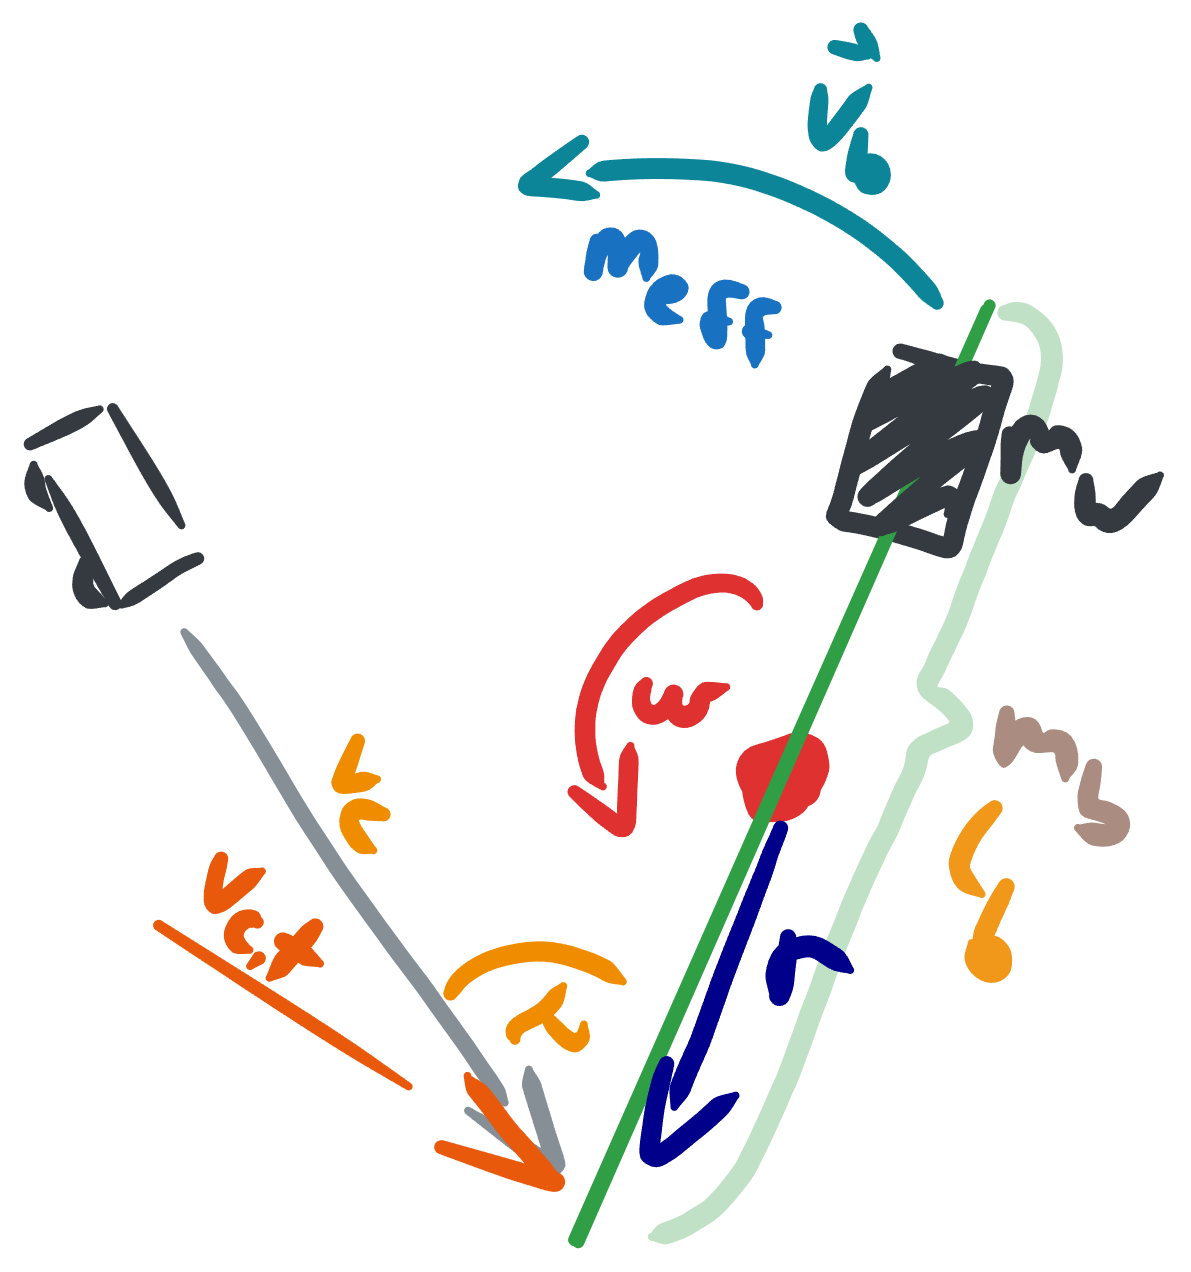
\includegraphics[width=0.38\textwidth]{resources/seq4/00_sketch.png}
	\vspace*{-5mm}
	\begin{flushright}
		{\scriptsize Eigenkreation; Gezeichnet in Excalidraw}
	\end{flushright}
	
	\captionsetup{
		labelfont=bf,
		textfont=footnotesize,
		skip=0pt
	}
	\caption{Einfache Skizze der Kollisionssequenz in Obersicht}
	\label{fig:04_sketch-whole}
	%\vspace{-10pt}
\end{wrapfigure}
\hyperref[fig:04_sketch-whole]{Abbildung~\ref*{fig:04_sketch-whole}} zeigt die für diese Sequenz relevanten Parameter. Einige davon können aus den Berechnungen der vorangegangenen Kapitel übernommen werden, während andere neu zu bestimmen sind.\\
\\
Der Betrag des Vektors $\vec{v_c}$ beschreibt die Gesamtfahrzeuggeschwindigkeit unmittelbar vor der Kollision. Die Berechnung von $\lvert \vec{v_c} \rvert$ wurde bereits im vorherigen Kapitel erläutert. Die exakte Richtung von $\vec{v_c}$ ließe sich aus den Rahmenbedingungen der ersten Sequenz bestimmen, ist für die folgenden Berechnungen jedoch nicht erforderlich, da lediglich der relative Einschlagwinkel zwischen Fahrzeug und Kranarm von Bedeutung ist. Dieser Winkel $\tau$ wurde bereits in Sequenz~1 %TODO reference
ermittelt und kann hier direkt übernommen werden. Mittels $\tau$ und $\vec{v_c}$ kann der Betrag des zum Kranarm tangential-verlaufenden Vektors $\vec{v_{c,t}}$ über $ \lvert\vec{v_{c,t}}\rvert = \sin(\tau) \cdot \lvert \vec{v_c} \rvert$ berechnet werden.
\\
Der Radius $r$ ist für die spätere Beschreibung der Dynamik von Wichtigkeit und stellt die Distanz des Kollisionspunktes zum Drehpunkt dar und wurde ebenfalls in Sequenz~1 %TODO
berechnet. 
\\
Zu Beginn ist die Winkelgeschwindigkeit $\omega$ des Krans null, die im weiteren Verlauf resultierende Winkelgeschwindigkeit stellt den zentralen Ermittlungsgegenstand dieses Kapitels dar.
\\
Für diese Sequenz müssen die Gesamtlänge des zum Drehpunkt symmetrischen Oberschwenkwerks, bestehend aus Ausleger und konterndem Gittermast, jedoch ohne Gegengewicht $l_b$, die Masse des Oberschwenkwerks ohne Ballast $m_b$, die Masse des Gegengewichts $m_w$ sowie der Abstand des Gegengewichts zum Drehpunkt $l_0$ neu abgeschätzt werden.


\subsection{Massenträgheitsmoment}
Zu Beginn soll das in der Rotationsdynamik zentrale Konzept des Massenträgheitsmoments betrachtet und berechnet werden. Das Trägheitsmoment nimmt im rotatorischen Bewegungskontext eine analoge Rolle zur Masse im translatorischen Fall ein \parencite{boege_gegenueberstellung}. Bei einem Stoßvorgang wird es benötigt, um das Verhältnis der Trägheiten der beteiligten Körper zu beschreiben.
\\
Das Gesamtträgheitsmoment eines Körpers ergibt sich aus der Summe aller mit ihm verbundenen Einzelträgheitsmomente \parencite{brenneke_schuster_ges-traegheit}:
$I_{ges} = \sum I_i$, wobei jedes Teilträgheitsmoment von der Masse und deren Abstand zum Drehpunkt abhängt \parencite{brenneke_schuster_ges-traegheit}, also $I_i = m_i \cdot r_i^2$.
Diese Beziehung gilt für Punktmassen. Bei einer homogenen, kontinuierlichen Massenverteilung muss stattdessen integriert werden \parencite{tipler_traegheitsmoment}. Der Körper wird dazu entlang der Rotationsachse in infinitesimal kleine Massenelemente $dm$ unterteilt. Jedes dieser theoretischen Massenelemente trägt gemäß der quadratischen Distanz zum Drehpunkt, wie bereits in \parencite{brenneke_schuster_ges-traegheit} beschrieben, zum Gesamtergebnis bei:
$I = \int r^2 \cdot dm$.
\\
Ein Massenelement ergibt sich aus der Dichte und einem infinitesimal kleinen Volumenelement, das sich wiederum als Produkt aus Querschnittsfläche und infinitesimaler Längen- bzw. Tiefendifferenz darstellen lässt: $dm = \rho \cdot dV = \rho \cdot A \cdot dx$.  
Da die homogene Dichte des Körpers als Quotient aus Gesamtmasse und Gesamtvolumen definiert ist, lässt sich für einen regelmäßig symmetrischen Körper mit konstantem Querschnitt schreiben: $\rho = \tfrac{m_{ges}}{l_{ges} \cdot A}$. Daraus folgt $\rho \cdot A = \tfrac{m_{ges}}{l_{ges}}$.  
In der Fachliteratur scheint es üblich, %TODO ref all sources
diesen Ausdruck als $\lambda := \tfrac{m_{ges}}{l_{ges}}$ zu bezeichnen. Damit kann im Ausdruck für das Massenelement $\rho \cdot A$ durch $\lambda$ ersetzt werden, sodass $dm = \lambda \cdot dx$ gilt. Das Trägheitsintegral lautet somit: $\int x^2 \cdot \lambda \cdot dx$.
\\
Im Folgenden wird das Eigenträgheitsmoment des Auslegersystems und dann zusätzliche Trägheitsmoment des Gegengewichts berechnet, um die beiden für einen Gesamtwert des Kranarms gemäß\parencite{brenneke_schuster_ges-traegheit} aufzusummieren. Diese Aufteilung erfolgt, da dann für beide Teilkomponenten eine homogene Masseverteilung angenommen werden kann, und mit dieser genaueren Parametrisierung eine bessere Schätzung möglich ist. 


\subsubsection{Ausleger}
\begin{wrapfigure}{r}{0.3\textwidth} %L
	\centering
	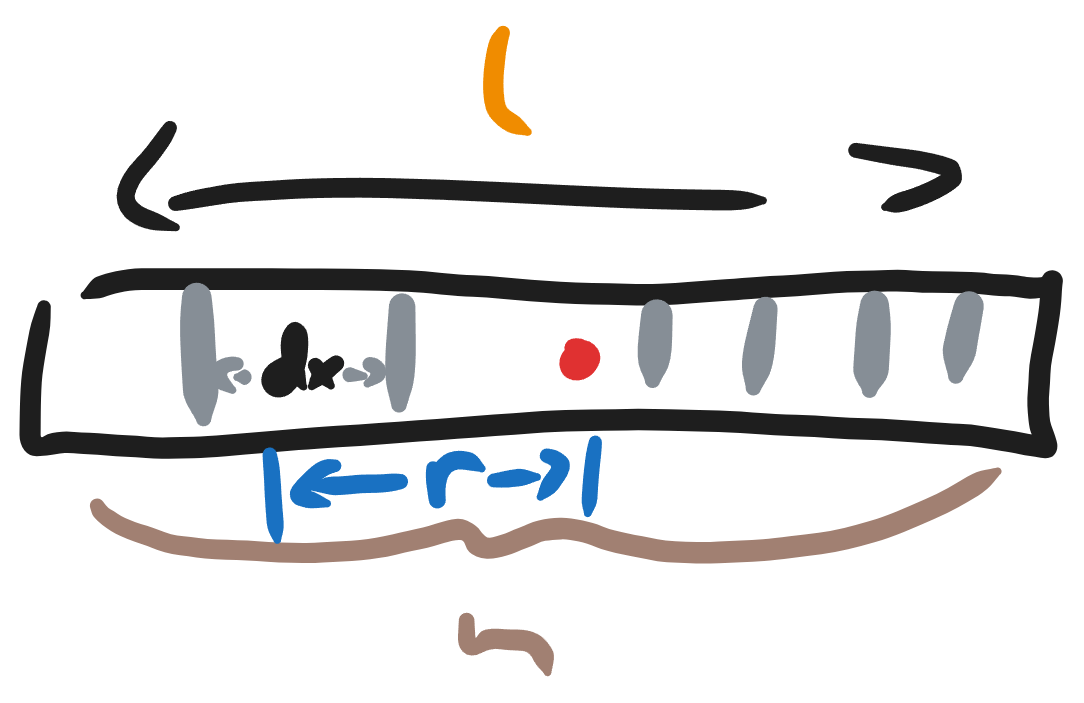
\includegraphics[width=0.28\textwidth]{resources/seq4/01_sketch_boom.png}
	\vspace*{-5mm}
	\begin{flushright}
		{\scriptsize Eigenkreation; Gezeichnet in Excalidraw}
	\end{flushright}
	
	\captionsetup{
		labelfont=bf,
		textfont=footnotesize,
		skip=0pt
	}
	\caption{Einfache Skizze des Auslegers}
	\label{fig:04_sketch_boom}
	%\vspace{-10pt}
\end{wrapfigure}
Für die Berechnung des Trägheitsmoments muss von der Drehpunkt aus über die gesamte Länge des Körpers integriert werden. Am Drehpunkt selbst gilt $x = 0$ bzw. $r = 0$. Im Falle des symmetrischen Oberschwenkwerks liegt der Drehpunkt in der Mitte der Integrationsachse, sodass von $-\tfrac{l}{2}$ bis $+\tfrac{l}{2}$ integriert werden muss.
\\
Da die lineare Massendichte $\lambda$ konstant ist, kann sie aus dem Integral herausgezogen werden, und das Trägheitsmoment lässt sich wie folgt darstellen:
\[
I \quad= \quad \lambda \cdot \int_{-l/2}^{+l/2} x^2 \, dx \quad = \quad \lambda \cdot \Big[ \frac{1}{3} \cdot x^3 \Big]_{-l/2}^{+l/2} \quad = \quad \lambda \cdot \left( \frac{1}{3} \cdot \left(\frac{l}{2}\right)^3 - \frac{1}{3} \cdot \left(-\frac{l}{2}\right)^3 \right)
\]
\[
I \quad = \quad \lambda \cdot \left( \frac{1}{3} \cdot \frac{l^3}{8} - \frac{1}{3} \cdot \left(-\frac{l^3}{2}\right) \right) \quad = \quad \lambda \cdot \left( \frac{l^3}{24} + \frac{l^3}{24} \right) \quad = \quad = \lambda \cdot \frac{l^3}{12}
\]
Mit $\lambda =  \tfrac{m}{l}$ folgt schließlich:
\[
I \; = \; \frac{m}{l} \cdot\frac{1}{12} \cdot  l^3 \quad = \quad \frac{1}{12} \cdot m \cdot l^2
\]

\subsubsection{Ballast}
\begin{wrapfigure}{r}{0.3\textwidth} %L
	\centering
	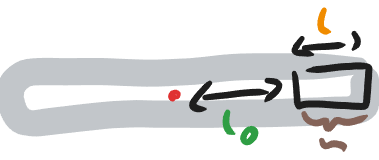
\includegraphics[width=0.28\textwidth]{resources/seq4/02_sketch_weight.png}
	\vspace*{-5mm}
	\begin{flushright}
		{\scriptsize Eigenkreation; Gezeichnet in Excalidraw}
	\end{flushright}
	
	\captionsetup{
		labelfont=bf,
		textfont=footnotesize,
		skip=0pt
	}
	\caption{Einfache Skizze des Gegengewichts}
	\label{fig:04_sketch_weight}
	%\vspace{-10pt}
\end{wrapfigure}
Für die Berechnung des Ballastgewichts bleibt das Integral dasselbe, aufgrund seiner exzentrischen Position allerdings, ändern sich die Integrationsgrenzen. Der in \hyperref[fig:04_sketch_weight]{~\ref*{fig:04_sketch_weight}} ersichtliche Versatz $l_0$ muss berücksichtigt werden:
\\[6pt]
$\displaystyle I \quad= \quad \lambda \cdot \int_{l_0}^{l+l_0} x^2 \, dx \quad = \quad \lambda \cdot \Big[ \frac{1}{3} \cdot x^3 \Big]_{l_0}^{l+l_0}$\\[5pt]
$\displaystyle = \lambda \cdot \left( \frac{1}{3} \cdot \left(l+l_0\right)^3 - \frac{1}{3} \cdot \left(l_0\right)^3 \right)$\\[5pt]
$\displaystyle = \lambda \cdot \frac{1}{3} \cdot \left(\left(l+l_0\right)^3 - \left(l_0\right)^3 \right)$\\[5pt]
$\displaystyle = \frac{m}{3\cdot l} \cdot \left(\left(l+l_0\right)^3 - \left(l_0\right)^3 \right)$
\\
\\
Alternativ kann zur Berechnung auch der Parallelachsensatz bzw. Satz von Steiner\parencite{kuchling_steiner} angewandt werden. Dieser besagt, dass das Trägheitsmoment eines Körpers um eine beliebige Achse, gleich dem Trägheitsmoment um eine parallele Achse durch seinen Massenmittelpunkt plus der Masse des Körpers multipliziert mit dem Quadrat des Abstands ist. Also: 
\[
I_{\mathrm{ges}} = \sum I_p + m_p \cdot s^2 \qquad \text{für einzelnen Körper: } I_{\mathrm{ges}} = I + m \cdot s^2
\]
Das Trägheitsmoment um die eigene Achse wurde oben schon berechnet und kann für das $I$ eingesetzt werden. $s$ ist der Massemittelpunkt des Gegengewichts, es ergibt sich aus der Summe des Abstands, und der halben Länge des exzentrischen Körpers.
\[
I_{\mathrm{ges}} = \left(\frac{1}{12} m \cdot l^2 \right) + m \cdot \left(l_0 + \frac{l}{2}\right)^2 \qquad I_{\mathrm{ges}} = \frac{1}{12} m \cdot l^2 + m \cdot \left(l_0 + \frac{l}{2}\right)^2
\]
Diese Formel ist äquivalent zum Ergebnis des Integrals.

\subsection{Reduzierte Masse}
%Kuchling 128
Nötig ist nun ein Modell, mit dessen Hilfe der translatorische Impuls des Fahrzeugs in eine rotatorische Bewegung des Kranarms überführt werden kann. Ein einfaches Gleichsetzen der Impulse und damit eine vollständige Energieübertragung entspräche jedoch nicht der physikalischen Realität, da der Stoßvorgang mit Energieverlusten und unterschiedlichen Trägheitsformen verbunden ist.
\\
Für die Beschreibung solcher Impulsübertragungen werden in der Physik verschiedene Stoßmodelle herangezogen. Im vorliegenden Fall bietet sich der \textit{teilelastische Stoß} als geeignete Näherung an. Damit dieses Modell angewendet werden kann, müssen die beteiligten Trägheiten in vergleichbare Größen überführt werden, das heißt, die rotatorische Trägheit des Kranarms muss in eine äquivalente translatorische Masse umgerechnet werden.
\\
Dieses Vorgehen basiert auf dem Konzept der reduzierten Masse. Unter Bezug auf \parencite{kuchling_red-masse} ergibt sich für die effektive Masse des Kranarms im Kontaktpunkt die Beziehung
\[
m_{\text{eff}} = \frac{I_{\text{kran}}}{r_{\text{kran}}^{2}},
\]
wobei $I_{\text{kran}}$ das Trägheitsmoment des Kranarms und $r_{\text{kran}}$ der Abstand zwischen Drehpunkt und Kollisionspunkt ist.
\\
Diese Verhältnismäßigkeit lässt sich plausibel herleiten, wenn man die kinetische Energie der Rotation $\tfrac{1}{2} I \omega^2$ mit der translatorischen Bewegungsenergie $\tfrac{1}{2} m_{\text{eff}} v^2$ gleichsetzt und in letzterer das $v$ als Bahngeschwindigkeit behandelt und durch seine Definition\(v = \omega \cdot r\) ersetzt. Daraus folgt $\tfrac{1}{2} I \omega^2 =\tfrac{1}{2} m_{\text{eff}} \cdot (\omega \cdot r)^2$. Im nächsten Schritt werden die Halben gekürzt, und das System durch $(\omega \cdot r)^2$ geteilt um auf $\frac{I \omega^2}{(\omega \cdot r)^2} = m_{\text{eff}}$ zu kommen. Im letzten Schritt können die $\omega^2$ gekürzt werden um die finale Form $m_{\text{eff}} = \frac{I}{r^2}$ zu erhalten. 
\\
Dadurch wird das Trägheitsmoment des gesamten Rotationssystems auf einen Punkt äquivalenter translatorischer Masse reflektiert.

\subsubsection{Gerader Zentrischer Stoß}
Mithilfe dieser reduzierten Masse lässt sich der Stoßvorgang, unter der Annahme eines fest gelagerten Drehpunkts des Kranarms, auf eine eindimensionale Impulsübertragung entlang der Stoßlinie reduzieren. Zur realistischeren Beschreibung des Energie- und Impulsaustauschs wird hierbei das Modell des teilelastischen Stoßes unter Verwendung eines Restitutionskoeffizienten $k$ herangezogen\parencite{kuchling_geschw-teilelastisch}.
\\
Diese Stoßzahl beschreibt das Verhältnis der relativen Geschwindigkeiten zweier Körper nach und vor dem Stoß und liegt definitionsgemäß im Intervall $0 \leq k \leq 1$. Ein Wert von $k = 1$ entspricht einem vollständig elastischen Stoß ohne Energieverlust, während $k = 0$ einem vollkommen inelastischen Stoß mit maximaler Energieabsorption entspricht \parencite{kuchling_geschw-teilelastisch}.
In der Praxis wird der Wert der Stoßzahl in der Regel empirisch durch Fall- oder Aufpralltests bestimmt\parencite{boege_stosszahl}. Für Stahl beträgt der Restitutionskoeffizient bei Raumtemperatur ($20\,^{\circ}\mathrm{C}$) typischerweise etwa $k = 0{,}7$, während er bei erhöhter Temperatur von etwa $1100\,^{\circ}\mathrm{C}$ auf rund $k = 0{,}35$ absinkt \parencite{boege_stosszahl}.
\\
Für die Berechnung wird ausschließlich die tangentiale Komponente der Fahrzeuggeschwindigkeit berücksichtigt, also jene Komponente, die senkrecht auf den Kranarm wirkt. Wie bereits in den vorangegangenen Kapiteln hergeleitet, ergibt sich deren Betrag zu $ \lvert\vec{v_{c,t}}\rvert = \sin(\tau) \cdot \lvert \vec{v_c} \rvert$.
\\
Unter Anwendung der Impuls-Geschwindigkeits-Gleichungen des teilweisen elastischen Stoßes\parencite{kuchling_geschw-teilelastisch} lässt sich die Geschwindigkeit des Fahrzeugs nach der Kollision $v'_{c,t}$ sowie die Bahngeschwindigkeit des Kranarms $v'_{b}$ am Kollisionspunkt mit Radius $r$ durch die effektive Masse des Kranarms $m_{\text{eff}}$ ausdrücken:
\[
v'_{c,t} = \frac{m_c \cdot v_{c,t} + m_{\text{eff}} \cdot v_b - m_{\text{eff}} \cdot (v_{c,t} - v_b) \cdot k}{m_c + m_{\text{eff}}},
\quad
v'_{b} = \frac{m_c \cdot v_{c,t} + m_{\text{eff}} \cdot v_b + m_c \cdot (v_{c,t} - v_b) \cdot k}{m_c + m_{\text{eff}}}.
\]
Da die Bahngeschwindigkeit des Kranarms zu Beginn null ist ($v_b = 0$), entfallen sämtliche Terme, in denen $v_b$ auftritt. Somit vereinfachen sich die Gleichungen entsprechend:
\[
v'_{c,t} = \frac{m_c \cdot v_{c,t} - m_{\text{eff}} \cdot (v_{c,t} - v_b) \cdot k}{m_c + m_{\text{eff}}},
\qquad
v'_{b} = \frac{m_c \cdot v_{c,t} + m_c \cdot (v_{c,t} - v_b) \cdot k}{m_c + m_{\text{eff}}}.
\]

\subsection{Kraftübertragungsmaximum} %TODO!!
Um eine Aussage über den Radius $r$ für eine optimale Kraftübertragung zu können muss herausgefunden werden unter welchen Bedingungen die Winkelgeschwindigkeit maximal wird. 

% Teil I: Definitionen und grundlegende Beziehungen
Die Winkelgeschwindigkeit $\omega$ des Krans nach dem Stoß ergibt sich aus der Bahngeschwindigkeit am Einschlagspunkt, die im Stoß beteiligte reduzierte Masse beinhaltet $r$
\[
\omega = \frac{v_b'}{r} \qquad m_{eff} = \frac{I}{r^2}
\]
Der Zusammenhang zwischen den Geschwindigkeiten vor und nach dem Stoß über den Stoßkoeffizienten $k$ ist folgendermaßen beschrieben. Da der Kran anfangs ruht fällt $v_b = 0$ weg, des Weiteren kann die Gleichung umgestellt werden, um später $v_{n,c}'$ durch seine Definition zu substituieren
\[
\left(v_{n,c} - v_b\right) \cdot k = v_b' - v_{n,c}' \qquad v_{n,c} \cdot k = v_b'-v_{n,c}' \qquad v_{n,c}' = v_b'- v_{n,c} \cdot k
\]
Durch die Beziehung der Impulserhaltung beim Stoß ergibt sich folgendes. $v_b = 0$ fällt wieder weg, anschließend kann $v_{n,c}'$ eingesetzt werden:
\[
v_{n,c} \cdot m_c + v_b \cdot m_c = v_{n,c}' \cdot m_c + v_b' \cdot m_{eff} \quad v_{n,c} \cdot m_c = v_{n,c}' \cdot m_c + v_b' \cdot m_{eff} \quad v_{n,c} \cdot m_c =\left(v_b'- v_{n,c} \cdot k \right)  \cdot m_c + v_b' \cdot m_{eff}
\]
Durch Anschließendes Ausmultiplizieren und $v_b'$ Ausklammern
\[
v_{n,c} \cdot m_c = - v_{n,c} \cdot k \cdot m_c \; + \; v_b'\cdot m_c \cdot m_c + v_b' \cdot m_{eff} \qquad v_{n,c} \cdot m_c = - v_{n,c} \cdot k \cdot m_c \; + \; v_b'\cdot \left( m_c + m_{eff}\right)
\]
$v_{n,c} \cdot k \cdot m_c$ Addieren, $m_c$ Ausklammern
\[
v_{n,c} \cdot m_c \; + \; v_{n,c} \cdot k \cdot m_c = v_b'\cdot \left( m_c + m_{eff}\right) \qquad v_{n,c} \cdot m_c \cdot \left(1+k\right) = v_b'\cdot \left( m_c + m_{eff}\right)
\]
Auflösen nach $v_b'$, anschließend kann $m_{eff} = \frac{I}{r^2}$ eingesetzt werden, um die Abhängigkeit des Radius $r$ einzuführen
\[
\frac{v_{n,c} \cdot m_c \cdot \left(1+k\right)}{ m_c + m_{eff}} = v_b' \qquad v_b' = \frac{v_{n,c} \cdot m_c \cdot (1 + k)}{k \cdot m_c + \frac{I}{r^2}}
\]
Mit $v_b' = \omega\cdot r$ ergibt sich:
\[
\omega\cdot r = \frac{v_{n,c} \cdot m_c \cdot (1 + k)}{k \cdot m_c + \frac{I}{r^2}} \qquad \omega= \frac{v_{n,c} \cdot m_c \cdot (1 + k)}{m_c + \frac{I}{r^2}}\cdot \frac{1}{r}
\]
Ausmultiplizieren:
\[
\omega= \frac{v_{n,c} \cdot m_c \cdot (1 + k)}{m_c \cdot r^2 + I}\cdot \frac{r^2}{r} \qquad = \frac{v_{n,c} \cdot m_c \cdot (1 + k)\cdot r}{m_c \cdot r^2 + I}
\]
Für optimale Einschlagsposition Winkelgeschwindigkeit maximieren: $\omega$ nach unserer gesuchten Größe $r$ ableiten und Nullstelle finden:
\[
\frac{d\omega}{dr} = \frac{v_{n,c} \cdot m_c \cdot (1 + k) \cdot (m_c \cdot r^2 + I) - v_{n,c} \cdot m_c \cdot (1 + k) \cdot r \cdot 2 \cdot m_c \cdot r}{(m_c \cdot r^2 + I)^2} \; \overset{!}{=} \; 0
\]
Faktor $v_{n,c} \cdot m_c \cdot (1 + k)$ ausklammern:
\[
\frac{d\omega}{dr} = \frac{v_{n,c} \cdot m_c \cdot (1 + k) \cdot \left[(m_c \cdot r^2 + I) - r \cdot 2 \cdot m_c \cdot r\right]}{(m_c \cdot r^2 + I)^2}
\]
Und Zähler vereinfachen:
\[
(m_c \cdot r^2 + I) - 2 \cdot m_c \cdot r^2 = m_c \cdot r^2 + I - 2 \cdot m_c \cdot r^2 = I - m_c \cdot r^2
\]
Somit:
\[
\frac{d\omega}{dr} = \frac{v_{n,c} \cdot m_c \cdot (1 + k) \cdot (I - m_c \cdot r^2)}{(m_c \cdot r^2 + I)^2}
\]
Für ein Extremum muss die Ableitung 0 ergeben, es wird nach einer Zählernullstelle gesucht: 
\[
\frac{d\omega}{dr} = 0 \qquad \underbrace{v_{n,c} \cdot m_c \cdot (1 + k)}_{>0} \cdot (I - m_c \cdot r^2) = 0
\]
Da $v_{n,c} \cdot m_c \cdot (1 + k) > 0$, folgt:
\[
I - m_c \cdot r^2 \overset{!}{=} 0 \qquad I = m_c \cdot r^2 \qquad r^2 = \frac{I}{m_c} \qquad r_{opt} = \pm \sqrt{\frac{I}{m_c}}
\]


\subsection{FEM Analyse}
cool :DAD:SD:ASDUIAFHwuihQAWEUIFRHWSEUIFASLJDFBN